\label{chapter-scenario-template}
\textbf{Created by:} Perawit Charoenwut \\
\textbf{Modified by:}

\subsection*{Scenario Objective}
This scenario illustrates how to represent a complete company structure with manufacturing and business divisions using the IOF core ontology. It focuses on:
\begin{itemize}
    \item Showing how business and manufacturing units coexist within one company
    \item Representing organizational hierarchy and relationships
    \item Distinguishing between business and manufacturing activities
    \item Capturing different organizational roles and functions
\end{itemize}

\subsection*{General Pattern Description}
A company can contain both business organizations and manufacturers as part of its structure. While all are types of Organization, they serve different functions and have different activities within the company structure.

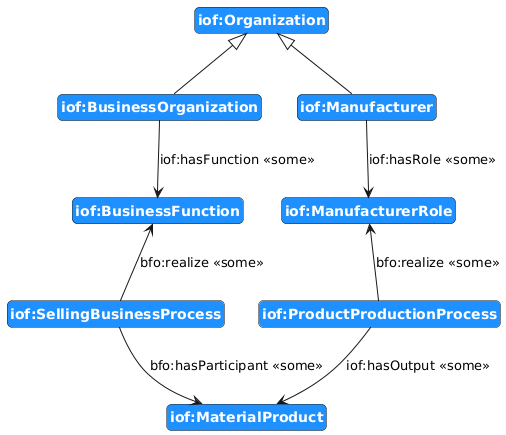
\includegraphics[scale=0.5]{scenarios/different-type-organizations/image/different-type-organizations-schema}

\subsection*{Use Case: }

The automobile company example demonstrates the distinction between business organizations and manufacturers.

\subsubsection*{Use-Case Pattern Description}

The company structure includes:
\begin{itemize}
    \item Parent company (Organization)
    \item Regional business divisions (BusinessOrganization)
    \item Manufacturing plants (Manufacturer)
    \item Sales and service divisions (BusinessOrganization)
\end{itemize}



\subsubsection*{Use-Case Example Data}
\begin{table}[h]
% \caption{}
\label{tab:organization-structure}
\resizebox{\columnwidth}{!}{%
\begin{tabular}{|l|l|l|l|l|}
\hline
Org\_ID & Org\_Type & Primary\_Activity & Functions \\ \hline
C\_001 & Organization & Corporate Management & Strategic Planning, Governance \\
M\_001 & Manufacturer & Vehicle Manufacturing & Assembly, Quality Control, R\&D \\
M\_002 & Manufacturer &  Parts Manufacturing & Parts Production, Testing \\
S\_001 & BusinessOrg &  Vehicle Sales & Marketing, Dealership Management \\
F\_001 & BusinessOrg &  Financial Services & Leasing, Insurance, Loans \\
L\_001 & BusinessOrg & Logistics Services & Transportation, Distribution \\ \hline
\end{tabular}%
}
\end{table}


\subsubsection*{Data Mapping}


\subsubsection*{Data Validation}
